
\documentclass[final]{beamer}

\usepackage[scale=1.24]{beamerposter} % Use the beamerposter package for laying out the poster


\usetheme{confposter} % Use the confposter theme supplied with this template

\setbeamercolor{block title}{fg=ngreen,bg=white} % Colors of the block titles
\setbeamercolor{block body}{fg=black,bg=white} % Colors of the body of blocks
\setbeamercolor{block alerted title}{fg=white,bg=dblue!70} % Colors of the highlighted block titles
\setbeamercolor{block alerted body}{fg=black,bg=dblue!10} % Colors of the body of highlighted blocks
% Many more colors are available for use in beamerthemeconfposter.sty

%-----------------------------------------------------------
% Define the column widths and overall poster size
% To set effective sepwid, onecolwid and twocolwid values, first choose how many columns you want and how much separation you want between columns
% In this template, the separation width chosen is 0.024 of the paper width and a 4-column layout
% onecolwid should therefore be (1-(# of columns+1)*sepwid)/# of columns e.g. (1-(4+1)*0.024)/4 = 0.22
% Set twocolwid to be (2*onecolwid)+sepwid = 0.464
% Set threecolwid to be (3*onecolwid)+2*sepwid = 0.708

\newlength{\sepwid}
\newlength{\onecolwid}
\newlength{\twocolwid}
\newlength{\threecolwid}
\setlength{\paperwidth}{48in} % A0 width: 46.8in
\setlength{\paperheight}{36in} % A0 height: 33.1in
\setlength{\sepwid}{0.024\paperwidth} % Separation width (white space) between columns
\setlength{\onecolwid}{0.22\paperwidth} % Width of one column
\setlength{\twocolwid}{0.464\paperwidth} % Width of two columns
\setlength{\threecolwid}{0.708\paperwidth} % Width of three columns
\setlength{\topmargin}{-0.5in} % Reduce the top margin size
%-----------------------------------------------------------

\usepackage{graphicx}  % Required for including images

\usepackage{booktabs} % Top and bottom rules for tables
\usepackage{exscale}
\usepackage{caption}
\captionsetup{labelformat=empty,labelsep=none}

%----------------------------------------------------------------------------------------
%	TITLE SECTION 
%----------------------------------------------------------------------------------------

\title{Deep Q-Learning With Recurrent Neural Networks} % Poster title

\author{Clare Chen, Vincent Ying, Dillon Laird} % Author(s)

\institute{Stanford, 2016} % Institution(s)

%----------------------------------------------------------------------------------------

\begin{document}

\addtobeamertemplate{block end}{}{\vspace*{2ex}} % White space under blocks
\addtobeamertemplate{block alerted end}{}{\vspace*{2ex}} % White space under highlighted (alert) blocks

\setlength{\belowcaptionskip}{2ex} % White space under figures
\setlength\belowdisplayshortskip{2ex} % White space under equations

\begin{frame}[t] % The whole poster is enclosed in one beamer frame

\begin{columns}[t] % The whole poster consists of three major columns, the second of which is split into two columns twice - the [t] option aligns each column's content to the top

\begin{column}{\sepwid}\end{column} % Empty spacer column

\begin{column}{\onecolwid} % The first column

%----------------------------------------------------------------------------------------
%	BACKGROUND
%----------------------------------------------------------------------------------------

\begin{alertblock}{Abstract}
    Deep reinforcement learning models have proven to be successful at learning
    control policies image inputs. However, they have struggled with learning
    policies that require longer term information. Recurrent neural network
    architectures have be used in tasks dealing with longer term dependencies
    between data points. We investigate these architectures to overcome the
    difficulties arising from learning policies with long term dependencies.
\end{alertblock}

%------------------------------------------------

\begin{block}{Introduction}
    \begin{itemize}
        \item Recent advances in reinforcement learning have led to human-level
              or greater performance on a wide variety of games (e.g. Atari 2600
              Games). 
        \item Deep Q-networks are limited in that they learn a mapping from a single
              previous state which consist of a small number of game screens.
        \item We explore the concepts of deep recurrent Q-networks (DRQN),
              and also a combination of recurrent neural network (RNN) and deep
              Q-network (DQN).
        \item In addition to standard RNN architectures, we also examine augmenting the RNN
              architecture with an attention mechanism. 
    \end{itemize}
\end{block}

%------------------------------------------------

\begin{figure}[h]
    \begin{minipage}{0.8\textwidth}
        \centering
        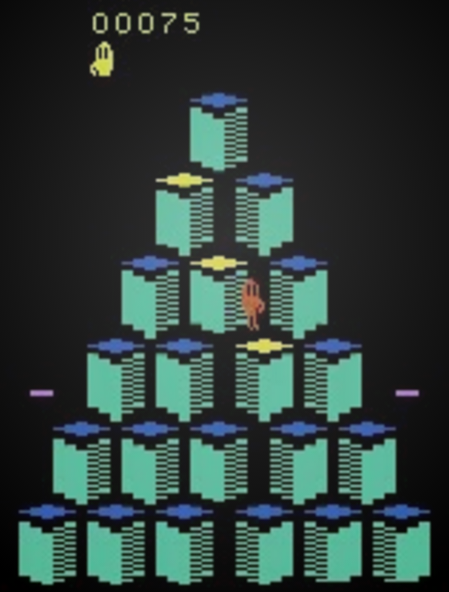
\includegraphics[scale=0.5]{Qbert}
        \centering
        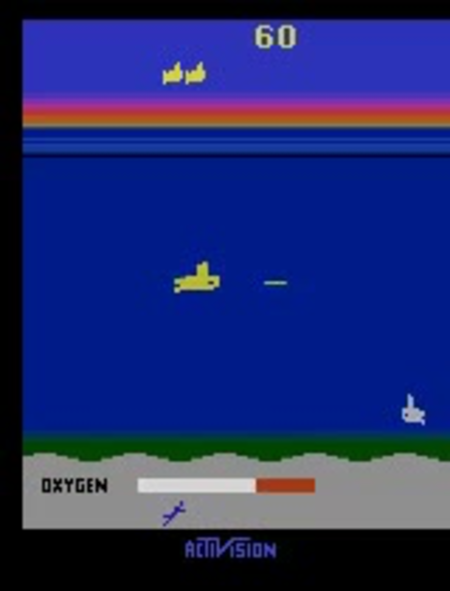
\includegraphics[scale=0.5]{Seaquest}
        \centering
        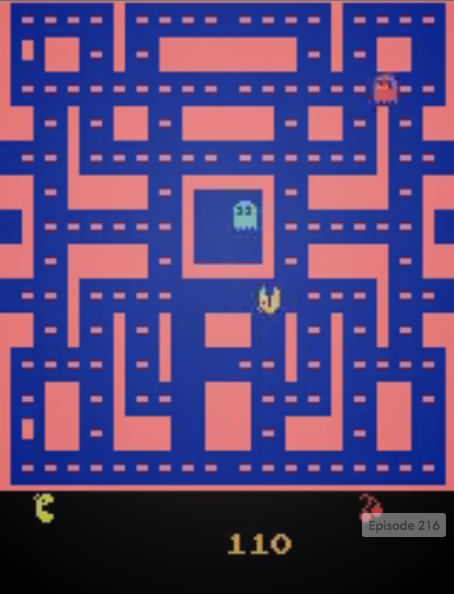
\includegraphics[scale=0.5]{MsPacman}
    \end{minipage}
    \caption{Q*bert, Seaquest, and Ms. Pac-Man}
\end{figure}

%----------------------------------------------------------------------------------------

\end{column} % End of the first column

\begin{column}{\sepwid}\end{column} % Empty spacer column

\begin{column}{\twocolwid} % Begin a column which is two columns wide (column 2)

\begin{columns}[t,totalwidth=\twocolwid] % Split up the two columns wide column

\begin{column}{\onecolwid}\vspace{-.6in} % The first column within column 2 (column 2.1)

%----------------------------------------------------------------------------------------
%	ALGORITHMS
%----------------------------------------------------------------------------------------

\begin{block}{Deep Recurrent Q-Learning}
\begin{itemize}
    \item The architecture of DRQN augments DQN's fully connected layer with a LSTM.
    \item We accomplish this by looking at the last $L$ states:
        $$ \{s_{t-(L-1)}, \dots, s_{t}\} $$
    \item We feed these into a convolution neural network (CNN) to get intermediate
        outputs and then send those through the RNN:
        $$\text{CNN}(s_{t-i}) = x_{t-i}$$
        $$\text{RNN}(x_{t-i}, h_{t-i-1}) = h_{t-i}$$
    \item The final output is used to predict the $Q$ value.
\end{itemize}

\end{block}

\begin{block}{Attention Deep Recurrent Q-Learning}
    \begin{itemize}
        \item In \textbf{linear attention}, we take the last $L$ hidden states and
            compute the inner product with learned vector $v_a$ and take a softmax:
            $$\{v_a^Th_{t-(L-1)}, \dots, v_a^Th_t\} \text{, }
              a_{t-i} = \text{softmax}(v_a^Th_{t-i})$$
    \end{itemize}
\end{block}

%----------------------------------------------------------------------------------------

\end{column} % End of column 2.1

\begin{column}{\onecolwid}\vspace{-.6in} % The second column within column 2 (column 2.2)

%----------------------------------------------------------------------------------------

%\begin{block}{Attention Deep Recurrent Q-Learning}
\begin{itemize}
        \item Then, we take a weighted sum of hidden states to get a context
            vector $c_t$ that is used to calculate $Q$:
            $$c_t = \sum_{i=0}^{L-1}a_{t-i}h_{t-i}$$
        \item In \textbf{global attention}, we use the current hidden state, $h_t$,
            to calculate the attention scores:
            $$\{{h_{t-(L-1)}}^Th_t, \dots, {h_{t-1}}^Th_t\} \text{, }
              a_{t-i} = \text{softmax}({h_{t-i}}^Th_t)$$
        \item We then compute a context vector similar to above and pass it through
            a final layer before it is used to compute $Q$:
            $$c_t = \sum_{i=1}^{L-1}a_{t-i}h_{t-i} \text{, }
              \tilde{h} = \tanh(W_a[h_t;c_t] + b_a)$$
\end{itemize}

\begin{figure}[h]
    \centering
    \includegraphics[scale=1.0]{DRQN_attn}
    \caption{Architecture of the Attention DRQN}
\end{figure}

%\end{block}

\end{column} % End of column 2.2

\end{columns} % End of the split of column 2 - any content after this will now take up 2 columns width

%----------------------------------------------------------------------------------------
%	EXPERIMENTS
%----------------------------------------------------------------------------------------

\begin{column}{\twocolwid}

\begin{block}{Experiments}
\end{block}

\end{column}

\begin{columns}[t,totalwidth=\twocolwid] % Split up the two columns wide column again

\begin{column}{\onecolwid} % The first column within column 2 (column 2.1)

\begin{itemize}
    \item Basic DQN
    \item Basic RDQN
\end{itemize}

%----------------------------------------------------------------------------------------

\end{column} % End of column 2.1

\begin{column}{\onecolwid} % The second column within column 2 (column 2.2)

\begin{itemize}
    \item RDQN with linear attention.
    \item RDQN with global attention.
\end{itemize}

%----------------------------------------------------------------------------------------

\end{column} % End of column 2.2

\end{columns} % End of the split of column 2

\begin{alertblock}{Box}
    Text or image?
\end{alertblock} 

\end{column} % End of the second column

\begin{column}{\sepwid}\end{column} % Empty spacer column

\begin{column}{\onecolwid} % The third column

%----------------------------------------------------------------------------------------
%	RESULTS
%----------------------------------------------------------------------------------------

\begin{block}{Results}

% SCORE TABLE
\begin{gather*}
	Q^{\ast}bert Scores
\end{gather*}

\begin{table}
    \vspace{2ex}
    \begin{tabular}{l l l}
        \toprule
            \textbf{Algorithms} & \textbf{Scores} \\
        \midrule
            Random & 157 \\
            Sarsa & 614 \\
            Contingency & 960 \\
            DQN & \textbf{1952} \\
            Human & 18900 \\
        \midrule
            HNeat Best & 1800 \\
            HNeat Pixel & 1325 \\
            DQN Best & \textbf{4500} \\
        \bottomrule
    \end{tabular}
\end{table}

\end{block}

%----------------------------------------------------------------------------------------
%	DISCUSSION
%----------------------------------------------------------------------------------------

\begin{block}{Discussion}

    \begin{itemize}
        \item Conclusions
        \item Future work
    \end{itemize}

\end{block}

%----------------------------------------------------------------------------------------

\end{column} % End of the third column

\end{columns} % End of all the columns in the poster

\end{frame} % End of the enclosing frame

\end{document}
